\testCom
{%Номер задачи
	3.161
}
{%Условие
	условие
}
{%Дано
	дано
}
{%Найти
	найти
}
{%Решение
	$I_\partial = \sqrt{\frac{1}{T} \int\limits_0^T i^2 \, dt}$\\
	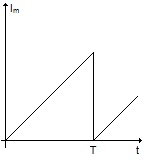
\includegraphics[height=30mm]{3_161.jpg}\\
	а) $I_0 = \sqrt{\frac{1}{T} \int\limits_0^T I \, dt} = \frac{I_m}{Q} \Rightarrow  I_m = 2 I_0$\\
	Очевидно, что $I(t) = kt, 0 \leqslant t \leqslant T,$ тогда \\
	$I_\partial = \sqrt{\frac{1}{T} \int\limits_0^T kt \, dt} = \frac{kT}{\sqrt{3}} = \frac{I_m}{\sqrt{3}} = \frac{2 I_0}{\sqrt{3}}$\\
	б) $I ~ \abs{\sin \omega t}, тогда T = \frac{\pi}{\omega}$\\
	$I(t) = I_m \sin \omega t, 0 < t < T$\\
	$I_0 = \frac{\omega}{\pi} I_m \int\limits_0^{\frac{\pi}{\omega}} \sin \omega t \, dt = \frac{\omega}{\pi} \cdot I_m \cdot 2 = \frac{2 \omega I_m}{\pi}$\\
	$I_\partial = \sqrt{\frac{1}{T} \int\limits_0^T I^2(t) \, dt} = \sqrt{\frac{\omega}{\pi} \cdot I_m^2 \int\limits_0^{\frac{\pi}{\omega}} \sin^2 \omega t \, dt} = 
	  \sqrt{\frac{\cancel \omega}{\pi} \cdot I_m^2 \int\limits_0^\pi \sin^2  t \, dt} = \frac{I_m}{\sqrt{\pi}} \sqrt{\frac{1}{2}  \int\limits_0^\pi (1 - \cancelto{0}{\cos 2t}) \omega t \, dt} = 
	  \frac{I_m}{\sqrt{2}} = \frac{\pi I_0}{2 \sqrt{2}}$\\
	
}

